\documentclass[a4paper,12pt]{article} % тип документа

% Поля страниц
\usepackage[left=2.5cm,right=2.5cm,
    top=2cm,bottom=2cm,bindingoffset=0cm]{geometry}
    
%Пакет дял таблиц   
\usepackage{multirow} 
    
%Отступ после заголовка    
\usepackage{indentfirst}


% Рисунки
\usepackage{floatrow,graphicx,calc}
\usepackage{wrapfig}

%%% Работа с картинками
\usepackage{graphicx}  % Для вставки рисунков
\graphicspath{{images/}}  % папки с картинками
\setlength\fboxsep{3pt} % Отступ рамки \fbox{} от рисунка
\setlength\fboxrule{1pt} % Толщина линий рамки \fbox{}
\usepackage{wrapfig} % Обтекание рисунков и таблиц текстом

% Создаём новый разделитель
\DeclareFloatSeparators{mysep}{\hspace{1cm}}

% Ссылки?
\usepackage{hyperref}
\usepackage[rgb]{xcolor}
\hypersetup{				% Гиперссылки
    colorlinks=true,       	% false: ссылки в рамках
	urlcolor=blue          % на URL
}


%  Русский язык
\usepackage[T2A]{fontenc}			% кодировка
\usepackage[utf8]{inputenc}			% кодировка исходного текста
\usepackage[english,russian]{babel}	% локализация и переносы

% Математика
\usepackage{amsmath,amsfonts,amssymb,amsthm,mathtools}

%%% Дополнительная работа с математикой
\usepackage{amsmath,amsfonts,amssymb,amsthm,mathtools} % AMS
\usepackage{icomma} % "Умная" запятая: $0,2$ --- число, $0, 2$ --- перечисление

% Что-то 
\usepackage{wasysym}


\begin{document}
\begin{center}
	\footnotesize{ФЕДЕРАЛЬНОЕ ГОСУДАРСТВЕННОЕ АВТОНОМНОЕ ОБРАЗОВАТЕЛЬНОЕ 			УЧРЕЖДЕНИЕ ВЫСШЕГО ОБРАЗОВАНИЯ}\\
	\footnotesize{МОСКОВСКИЙ ФИЗИКО-ТЕХНИЧЕСКИЙ ИНСТИТУТ\\(НАЦИОНАЛЬНЫЙ 			ИССЛЕДОВАТЕЛЬСКИЙ УНИВЕРСИТЕТ)}\\
	\footnotesize{ФИЗТЕХ-ШКОЛА ФИЗИКИ И ИССЛЕДОВАНИЙ им. ЛАНДАУ\\}
	\hfill \break
	\hfill \break
	\hfill \break
	\hfill \break
\end{center}

\begin{center}   
    \hfill \break
	\hfill \break
	\hfill \break
	\hfill \break    \hfill \break
	\hfill \break
	\hfill \break
	\hfill \break
    \hfill \break
    \hfill \break
	\hfill \break
	\large{Лабораторная работа № 2.2.3\\\textbf{Измерение теплопроводности воздуха при атмосферном давлении}}\\
	\begin{flushright}
		Плотникова Анастасия Александровна\\
		Группа Б02-406
	\end{flushright}
	\hfill \break
	\hfill \break
	\hfill \break
\end{center}
\hfill \break
\hfill \break
\hfill \break
\hfill \break
\hfill \break
\hfill \break
\hfill \break
\hfill \break
\hfill \break
\hfill \break
\hfill \break
\hfill \break
\hfill \break
\begin{center}
	Долгопрудный, 2025 г.
\end{center}
\thispagestyle{empty}
\newpage
	\textbf{Цель работы:}\\ 
  измерить коэффициент теплопроводности воздуха при атмосферном
давлении в зависимости от температуры
	\hfill \break
	
	\textbf{В работе используются:}\\ 
  цилиндрическая колба с натянутой по оси нитью; \\
  термостат; \\
  вольтметр и амперметр (цифровые мультиметры); \\
  эталонное сопротивление; \\
  источник постоянного напряжения; \\
  реостат (или магазин сопротивлений)

\section*{Теоретическая справка}

\textbf{Теплопроводность} — это процесс передачи тепловой энергии от нагретых частей системы к холодным за счёт хаотического движения частиц среды. 

\textbf{Закон Фурье}. Плотность потока энергии $\vec{q}$ (Вт/м$^2$) — количество теплоты, переносимое через единичную площадку в единицу времени — пропорциональна градиенту температуры $\nabla T$:
\begin{equation}
    \vec{q} = -\kappa \cdot \nabla T, \label{eq:fourier}
\end{equation}
где $\kappa$ (Вт/(м$\cdot$К)) — коэффициент теплопроводности.

Оценка для коэффициента теплопроводности газов:
\begin{equation}
    \kappa \sim \lambda \bar{v} \cdot n c_V, \label{eq:kappa_estimate}
\end{equation}
где:\\ 
$\lambda$ — длина свободного пробега молекул газа,\\
$\bar{v} = \sqrt{\dfrac{8k_B T}{\pi m}}$ — средняя скорость теплового движения молекул, \\
$n$ — концентрация (объёмная плотность) газа, \\
$c_V = \dfrac{i}{2}k_B$ — теплоёмкость при постоянном объёме на одну молекулу, \\
$i$ — эффективное число степеней свободы молекулы. \\

Формула \eqref{eq:kappa_estimate} даёт лишь оценку по порядку величины и правильную функциональную зависимость. В учебной литературе часто приводится формула с численным коэффициентом $\frac{1}{3}$. Но это не более, чем оценка. 
\[
    \kappa = \frac{1}{3} \lambda \bar{v} \cdot n c_V.
\]

Длина свободного пробега может быть оценена как $\lambda = \dfrac{1}{n \sigma}$, где $\sigma$ — эффективное сечение столкновений молекул друг с другом.

Тогда из \eqref{eq:kappa_estimate} видно, что коэффициент теплопроводности газа не зависит от плотности газа и определяется только его температурой. В простейшей модели твёрдых шариков $\sigma = \text{const}$, и коэффициент теплопроводности пропорционален корню из абсолютной температуры:
\[
    \kappa \propto \frac{\bar{v}}{n} \propto \sqrt{T}.
\]

На практике эффективное сечение $\sigma(T)$ следует считать медленно убывающей функцией $T$, поскольку при увеличении $T$ молекулы движутся быстрее и проводят меньше времени во интенсивном взаимном взаимодействии, что снижает вероятность эффективного столкновения.

\medskip

Рассмотрим стационарную теплопередачу от тонкой нити (радиус $r_1$, длина $L$), расположенной вдоль оси цилиндра (радиус $r_0$), к его стенкам с постоянной температурой $T_0$. В нити выделяется мощность $Q$. При $L \gg r_0$ теплоотвод через торцы пренебрежимо мал, поток тепла направлен радиально, параметры зависят только от $r$.

Скалярная форма закона Фурье:
\begin{equation}
    q = -\kappa \frac{dT}{dr}.
\end{equation}

Полный поток через цилиндрическую поверхность:
\begin{equation}
    Q = -2\pi r L \cdot \kappa \frac{dT}{dr} = \text{const}.
\end{equation}

При малом перепаде температур $\Delta T = T_1 - T_0$ и $\kappa \approx \kappa(T_0)$, интегрирование даёт:
\begin{equation}
    Q = \frac{2\pi L \kappa \Delta T}{\ln(r_0 / r_1)}.
\end{equation}

Видно, что закон Ньютона выполняется, то есть поток тепла через систему пропорционален разности температур в
ней.

\subsection*{Оценка времени установления равновесия}

При изменении температуры или мощности нагрева система переходит в новое стационарное состояние за конечное время~$\tau$. Оценим его по порядку величины для плоского слоя толщиной~$a$ и площадью~$S$, заполненного газом при постоянном давлении. 

Температурный скачок~$\Delta T$ вызывает тепловой поток:
\[
q \sim \kappa \frac{\Delta T}{a}.
\]

Для нагрева слоя на~$\Delta T$ требуется тепло:
\[
Q_\text{необх.} = n S a \cdot c_P \Delta T.
\]

Поступившее за время~$\tau$ тепло:
\[
Q = q S \tau = \kappa \frac{\Delta T}{a} S \tau.
\]

Приравнивая, получаем оценку:
\[
\tau \sim \frac{a^2}{\chi}, \quad \text{где} \quad \chi = \frac{\kappa}{n c_P}.
\]
Величина~$\chi$ — температуропроводность, определяет скорость теплового выравнивания. Для воздуха при Н.У. $\chi \sim 0{,}2~\text{см}^2/\text{с}$, при $a \sim 1~\text{см}$ получаем~$\tau \sim 5~\text{с}$.

\subsection*{Пределы применимости теории}

Закон Фурье может нарушаться, если характерные размеры задачи сравнимы с длиной свободного пробега~$\lambda$. Тогда возникает, например, температурный скачок между нитью и газом. В данной работе этим можно пренебречь, так как при атмосферном давлении:
\[
\lambda \sim 10^{-5}~\text{см} \ll r_\text{нити}.
\]

Также возможны и другие механизмы теплопередачи: конвекция и излучение.

\textbf{Конвекция:} подавляется вертикальной ориентацией установки (градиент температуры горизонтален).

\textbf{Излучение:} становится заметным при сильном перегреве нити. Мощность излучения по закону Стефана–Больцмана:
\[
Q_{\text{изл}} = \epsilon \sigma_S S (T_1^4 - T_0^4) \approx 4 \epsilon \sigma_S S T_0^3 \Delta T,
\]
где $\sigma_S = 5{,}67 \cdot 10^{-8}~\text{Вт}/(\text{м}^2\cdot\text{К}^4)$, $\epsilon \sim 0{,}1 \div 0{,}2$ — коэффициент черноты для полированных металлов. В условиях опыта вклад излучения мал.



\section*{Экспериментальная установка}

Схема установки изображена на рисунке (\ref{fig:setup}). 

\begin{figure}[h!]
  \centering
  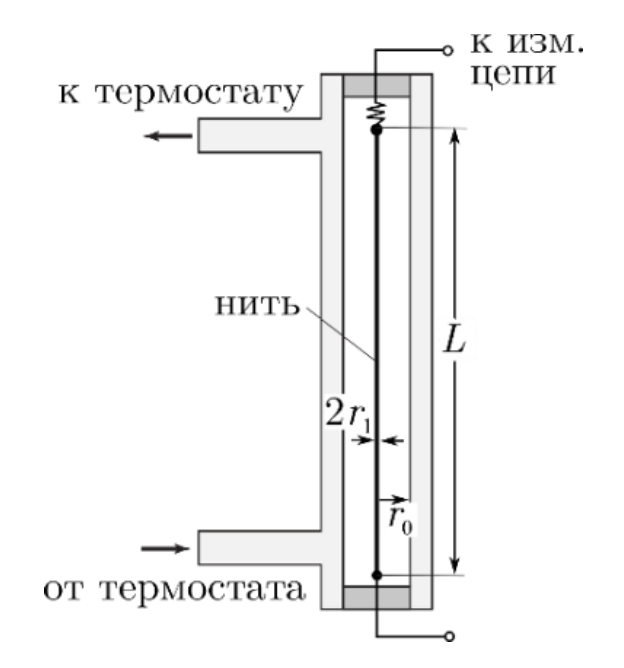
\includegraphics[scale = 0.5]{setup.png}
  \caption{Схема установки}
  \label{fig:setup}
\end{figure}

Внутри вертикально расположенной полой цилиндрической трубки диаметром $2r_0 \sim 1$ см размещена металлическая нить диаметром $2r_1 \sim 0{,}05$ мм и длиной $L \sim 40$ см. Трубка заполнена воздухом и соединена с атмосферой. Стенки охлаждаются водой из термостата, поддерживающего температуру $t_0$. Вертикальное расположение исключает конвекцию.

Нить служит источником тепла и термометром сопротивления. По закону Джоуля–Ленца:
\[
Q = UI, \qquad R = \frac{U}{I}.
\]

Сопротивление $R(t)$ однозначно связано с температурой. При $Q \to 0$ температура нити $t_1 \to t_0$, что позволяет определить зависимость $R(t)$. Альтернативно, используется табличная зависимость удельного сопротивления от температуры.

Относительное изменение сопротивления при $\Delta t = 1^\circ$C обычно составляет $0.2\% \pm 0.6\%$, поэтому измерения требуют высокой точности (погрешность менее $0{,}1\%$).

На рисунке (\ref{fig:curcuit}) приведены два варианта электрической схемы установки.

\begin{figure}[h!]
  \centering
  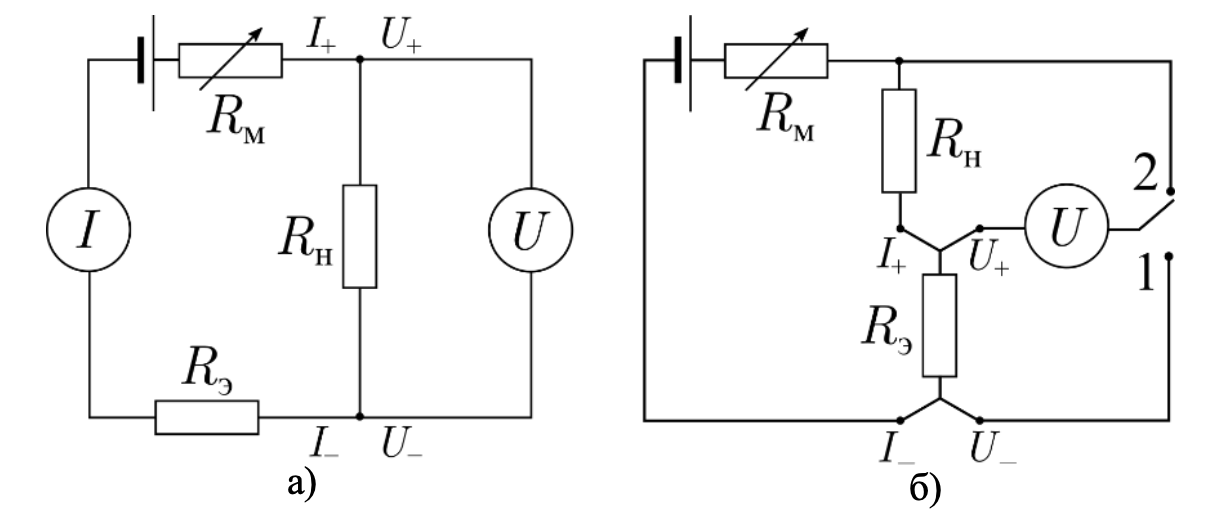
\includegraphics[scale = 0.5]{curcuit.png}
  \caption{Варианты электрических схем измерения сопротивления нити и мощности нагрева: а) с двумя мультиметрами, б) с одним вольтметром и эталонным сопротивлением}
  \label{fig:curcuit}
\end{figure}

В обеих схемах ток регулируется реостатом $R_\text{м}$, подключённым последовательно с источником питания.

\subsection*{Методика измерений}

Измерение сопротивления нити с током приводит к самонагреву:
\[
Q = I^2 R.
\]

Для исключения систематической ошибки используют метод экстраполяции: строится нагрузочная кривая $R(Q)$, и по её пересечению с осью $Q=0$ находят сопротивление $R_0$, соответствующее температуре окружающей среды $t_0$.

При этом можно аппроксимировать зависимость:
\[
R(t) = R_{273} \cdot (1 + \alpha t),
\]
где $R_{273}$ — сопротивление при $0^\circ$C, $\alpha$ — температурный коэффициент сопротивления:
\[
\alpha = \frac{1}{R_{273}} \frac{dR}{dt}.
\]

Измерения $R(Q)$ при разных $t_0$ дают $R(t)$. По наклонам кривых и формуле (\ref{}) определяется теплопроводность $\kappa$.

\section*{Ход работы}
\begin{center}
  \textsf{I. Подготовка к эксперименту}
\end{center}

\begin{enumerate}
    \item Проведём предварительные расчёты параметров опыта. 
    
    Для этого зафиксируем параметры установки. Нить платиновая.
    $R^{Pt}_0 \approx 20 \, \Omega$ — сопротивление нити при комнатной температуре; \\
    $2r_0 = (0.7 \pm 0.1) \, \text{см} = (7 \pm 1) \, \text{мм}$ — внутренний диаметр цилиндрической трубки;
    $2r_1 = (0.05 \pm 0.01) \text{мм}$ — диаметр платиновой нити;
    $L \approx 0.40 м$ — длина нити;
    $\Delta T = 30 \, K$ — максимальный перегрев нити относительно термостата при напряжении источника питания;
    $\kappa \approx 25 \frac{\text{мВт}}{\text{м}\cdot\text{K}} = 25 \cdot 10^{-3} \, \frac{\text{Вт}}{\text{м}\cdot\text{K}}$ — коэффициент теплопроводности воздуха (для оценки максимальной мощности нагрева). 


    
    Приняв максимально допустимый перегрев нити относительно термостата равным $\Delta t_{\text{max}} = 30^\circ$C, оценим максимальную мощность нагрева $Q_{\text{max}}$ [мВт] (см. формулу (5)), которую следует подавать на нить. 
\begin{itemize}
  \item Для оценки коэффициента теплопроводности воздуха примем $\kappa \sim 25$ мВт/(м$\cdot$К).
  \item По вычисленной мощности и приближенному значению сопротивления нити $R_n$ (см. техническое описание установки), определим соответствующие значения максимального тока $I_{\text{max}}$ и максимального напряжения $U_{\text{max}}$ на ней. 
  \item Перед переходом к измерениям обязательно покажем результаты расчёта преподавателю (или лаборанту). При дальнейшей работе во избежание перегрева нити не допустим превышения данных параметров.
\end{itemize}
  
  ВНИМАНИЕ! Во избежание перегорания нити не увеличим напряжение на источнике питания $\mathcal{E}$ выше указанного на установке!

\item Подготовим экспериментальную установку.
\begin{itemize}
  \item Проверим, что измерительная цепь соответствует схеме рис. 3 (а или б).
  \item На магазине сопротивлений (или на реостате) установим такое сопротивление $R_m$, чтобы ток в цепи при её замыкании был минимален ($R_m \geq 10$ кОм).
  \item Включим вольтметр и амперметр и настроим режимы их работы (по техническому описанию к установке).
  \item Включим источник питания; проверим, что он работает в режиме источника напряжения, и что напряжение на нём не превышает максимально допустимое (указано на установке).
  \item Включим термостат и убедимся, что вода в нём находится при комнатной температуре (измеренной по комнатному термометру, расположенному по возможности ближе к экспериментальной установке); при необходимости нагреем/охладим термостат.
\end{itemize}

\begin{center}
  \textsf{II. Проведение измерений}
\end{center}

    \item При фиксированной температуре термостата измерим зависимость сопротивления нити $R_n = \frac{U}{I}$ от подаваемой на неё мощности $Q = U I$ — нагрузочную кривую $R_n(Q)$.
    \begin{itemize}
      \item Измерения проведём для 9–10 значений тока $I$ через нить от 0 до $I_{\text{max}}$.
      \item Постараемся подбирать такие значения сопротивления магазина $R_m$, чтобы мощность нагрева нити $Q = I^2 R_n$ возрастала приблизительно равномерно в диапазоне от 0 до $Q_{\text{max}}$.
      \item Ток следует наращивать монотонно, постепенно уменьшая сопротивление магазина сопротивлений $R_m$. Перед фиксацией показаний дождёмся установления теплового равновесия (время ожидания $\sim 30$ с): показания мультиметров должны быть стационарны (флуктуировать вблизи постоянного значения). При измерениях рекомендуется не только записывать показания мультиметров (напряжение $U$ и ток $I$), но и сразу вычислять $R_n$ и $Q$.
      \item В процессе измерений контролируем постоянство температуры термостата. Если за время измерений температура термостата изменилась более чем на 0,1℃, опыт рекомендуется переделать.
    \end{itemize}

    \item По окончании измерений нагрузочной кривой установим минимальный ток через нить, переведя значение магазина сопротивления $R_m$ на 10 кОм или более. В дальнейшем будем возвращать магазин сопротивлений в это положение после каждого измерения нагрузочной кривой.
    \item Проведём измерения нагрузочных кривых согласно п. 3–4 для 5–7 температур термостата в диапазоне от комнатной до 80℃. Приступим к измерениям при новой температуре лишь после установления стационарного состояния (время ожидания не менее 15 минут).
    \item После завершения измерений выключим блок питания и цифровые мультиметры. На магазине сопротивлений (реостате) $R_m$ установим максимальное сопротивление ($\geq 10$ кОм). Поставим термостат на охлаждение до комнатной температуры (питание термостата не выключать).

\begin{center}
  \textsf{III. Обработка результатов измерений}
\end{center}

    \item Для каждой температуры термостата построим график зависимости сопротивления нити от мощности $R(Q)$. 
    
    Убедимся в линейности полученных зависимостей. Проведём наилучшие прямые и определим точки их пересечения с осью ординат $R_0$ (при $Q \to 0$ температура нити совпадает с температурой термостата) и угловые коэффициенты наклона $\frac{dR}{dQ}$. 
    
    Оценим погрешности найденных значений.
    \item Пользуясь значениями $R_0$ из п. 6, построим график зависимости сопротивления нити от её температуры $R(T)$. Убедимся в линейности полученной зависимости. Построим наилучшую прямую и определим её наклон $\frac{dR}{dT}$. Оценим погрешности.
    
    Сравним температурный коэффициент сопротивления материала нити $\alpha = \frac{1}{R_{273}} \frac{dR}{dT}$ с табличным (если материал проволоки известен).
    \item Используя угловой коэффициент температурной зависимости сопротивления п. 8 и угловые коэффициенты нагрузочных прямых из п. 7, вычислим наклон зависимости выделяющейся на нити мощности $Q$ от её перегрева $\Delta T$ относительно стенок:
    \[
    \frac{dQ}{d(\Delta T)} = \frac{\frac{dR}{dT}}{\frac{dR}{dQ}}.
    \]
    Отсюда, с учётом формулы (5), найдём коэффициенты теплопроводности газа $\kappa$ для каждой температуры термостата $T_0$. Оценим погрешности полученных результатов.
    \item Построим график зависимости теплопроводности воздуха от температуры газа $\kappa(T)$. Сравним результаты с табличными данными.
    
    Предполагая, что $\kappa$ степенным образом зависит от абсолютной температуры $T$: 
    \[
    \kappa \propto T^\beta,
    \]
    построим график в двойном логарифмическом масштабе (в координатах $\ln \kappa$ против $\ln T$) и определим из него показатель степени $\beta$. 

    Сравним результат с предсказанием теории, считая молекулы твёрдыми шариками. Сделаем вывод о зависимости сечения столкновений молекул от температуры.
\end{enumerate}

\section*{Вывод}
\end{document}

\begin{comment}
\section*{Ход работы}
\begin{center}
  \textsf{I. Подготовка к эксперименту}
\end{center}

\begin{enumerate}
    \item Проведём расчёты параметров опыта.
    \begin{itemize}
      \item Примем перегрев нити $\Delta t_{\text{max}} = 30^\circ$C и оценим максимальную мощность $Q_{\text{max}}$.
      \item Оценим максимальный ток $I_{\text{max}}$ и напряжение $U_{\text{max}}$ по значению сопротивления нити $R_n$.
      \item Покажем результаты расчёта преподавателю.
    \end{itemize}
  
    ВНИМАНИЕ! Не увеличим напряжение выше допустимого значения!

\item Подготовим экспериментальную установку.
\begin{itemize}
  \item Проверим схему подключения и установим сопротивление на магазине $R_m$ на 10 кОм.
  \item Настроим вольтметр и амперметр согласно техническому описанию.
  \item Включим источник питания и термостат, проверим температуру в термостате.
\end{itemize}

\begin{center}
  \textsf{II. Проведение измерений}
\end{center}

    \item Измерим зависимость сопротивления нити $R_n = \frac{U}{I}$ от мощности $Q = U I$ для 9–10 значений тока $I$.
    \begin{itemize}
      \item Регулярно наращиваем ток и уменьшаем сопротивление $R_m$.
      \item Проверим стабилизацию показаний мультиметров перед записью.
      \item Контролируем стабильность температуры термостата.
    \end{itemize}

    \item По завершении измерений установим минимальный ток через нить и вернём сопротивление $R_m$ на 10 кОм.
    \item Повторим измерения для 5–7 температур термостата.
    \item Выключим блок питания и мультиметры по завершении работы, установим максимальное сопротивление на $R_m$.
    
\begin{center}
  \textsf{III. Обработка результатов}
\end{center}

    \item Построим график зависимости $R(Q)$ для каждой температуры, оценим линейность, найдем $R_0$ и $\frac{dR}{dQ}$.
    \item Построим график зависимости $R(T)$ и определим наклон $\frac{dR}{dT}$.
    \item Вычислим наклон зависимости $Q(\Delta T)$ и определим коэффициент теплопроводности $\kappa$ для разных температур.
    \item Построим график зависимости $\kappa(T)$ и определим показатель степени $\beta$.
\end{enumerate}
\end{comment}